\numberwithin{equation}{section}
% A page that holds only floats starts them at the top instead of centering them.
\makeatletter\setlength{\@fptop}{0pt}\makeatother

\newpage

\section{Method details}
\label{app:method}

This appendix collects the details of \Cref{sec:method} that the main text summarizes or leaves out, in the order of its
subsections. For each part it states the
constants, schedules, scoring rules, and examples, explains why they are
designed as they are, and names the step of \Cref{alg:mirix} they belong to.

\subsection{Memory types, routing, and writing}
\label{app:method-routing}

The Meta Memory Manager is the first call of the write path
(\Cref{alg:mirix}, line~\ref{alg:route}). The router reads the input and
selects the memory types it updates. Each selected writer then reads the
current store \(P_u^{t-1}\) and produces a record that line~\ref{alg:commit}
commits to the evidence plane before any graph work begins. Formally, each
input \(x_t\) is mapped to a subset of six specialized writers,
\begin{equation}
    \begin{aligned}
    \mathcal K_t&=R_\theta(x_t),\\
    m_t^{(k)}&=W_k(x_t,P_u^{t-1}),\quad k\in\mathcal K_t,
    \end{aligned}
    \label{eq:routing}
\end{equation}
and each writer owns the schema and update operations of one memory type. Both
steps of \eqref{eq:routing} are language-model calls, which is why the router
and the writers carry the \(\star\) mark in \Cref{alg:mirix}.
\Cref{tab:memory-types} lists the six types.

\suppressfloats[t]
\begin{table}[t]
\centering
\caption{The six memory types of \ours and their roles.}
\label{tab:memory-types}
\small
\begin{tabular}{lll}
\toprule
Memory & Primary role & Hypergraph indexed \\
\midrule
Core & persistent user and agent state & no \\
Episodic & time-grounded occurrences & yes \\
Semantic & durable facts and concepts & yes \\
Procedural & executable workflows & no \\
Resource & documents and multimodal artifacts & no \\
Knowledge Vault & sensitive verbatim values & no \\
\bottomrule
\end{tabular}
\end{table}

The separation is functional. Only episodic and semantic memory are indexed by
the hypergraph, because they hold the event and relational evidence that
cross-memory traversal needs. The other types keep their direct, type-specific
retrieval paths. Core memory holds the persistent state of the user and the
agent, procedural memory holds the skills that \Cref{sec:autodream} refines,
resource memory holds documents and multimodal artifacts, and the knowledge
vault holds sensitive verbatim values. Each of them is read through its own typed path rather than through the graph.
In \Cref{alg:mirix}, the test \(k\in\{\mathrm{episodic},\mathrm{semantic}\}\) is the only step of the write
path that depends on whether a record is graph-indexed. In \Cref{fig:mirix-user-centric}, both user turns are
routed to the episodic and semantic writers.

\paragraph{Source-faithful writing.}
Before a record reaches the graph extractor, the writer prompts of our runs ask
the episodic and semantic writers to keep complete lists, names, counts, titles,
locations, and dates in the record's details instead of replacing them with a
topical gist. Episodic writers store the time an event happened rather than the
time it was mentioned, and they store a planned event with its planned date.

\paragraph{Write ordering.}
The write to the vector database commits before graph construction begins
(line~\ref{alg:commit}). Graph extraction
is a fail-soft indexing hook, so a graph failure is logged but never rolls back
a stored memory. The evidence plane is thus the durable system of record rather
than a side effect of graph construction.

\subsection{Anchor admission, canonicalization, and frame extraction}
\label{app:method-graph}

This part details lines~\ref{alg:extract} to~\ref{alg:upsert} of
\Cref{alg:mirix}, which turn a committed episodic or semantic record into the
anchors and frames of \Cref{sec:hypergraph}.

\paragraph{Anchor keys and admission.}
The key \(\kappa(n)\) of an anchor name normalizes case, punctuation, articles
and other function words, word order, and conservative singular and plural
variants while keeping numbers. In the code it lowercases the name, replaces
punctuation with spaces, drops a fixed list of eleven articles and function
words, singularizes tokens of at least four letters, and sorts the remaining
tokens, so that \emph{Mobile App} and \emph{Mobile Apps} share one key. The key
is deliberately conservative. Numbers and dates are preserved, so \emph{10 Gallons} and \emph{20 Gallons}
stay distinct, and only plural endings are normalized, so \emph{Training} and
\emph{Trains} stay apart. A
single admission gate rejects generic filing terms, such as \emph{advice},
\emph{details}, \emph{information}, \emph{plan}, and \emph{tips}, and
dialogue-role pseudo-entities such as \emph{user} and \emph{assistant}, and it
keeps at most 16 anchors for an episodic record and 18 for a semantic one. The
caps bound the anchor space of a user, and they are sized for the arguments of
an assertion rather than for a bag of keywords, so that one frame with seven
arguments does not exhaust them. The gate is the \textsc{Admit} call of
\Cref{alg:mirix}, and because it runs on the canonical key, one entry such as
\emph{user} also blocks \emph{User}, \emph{Users}, and \emph{the user}.

\paragraph{Registry-guided canonicalization.}
For every extracted entity, approximate nearest-neighbor search retrieves up to four existing anchors of the user whose cosine
similarity is at least \(0.72\), and one language-model call per record makes a
conservative same-entity decision for all of its entities. The vector index
scores a pair by \((1+\cos)/2\), so the thresholds in the code are 0.86 here
and 0.93 for AutoDream (\Cref{app:method-autodream}). The call is instructed
not to merge different quantities, different days or months, different form or
model codes, or related but distinct concepts. Canonicalization runs before the admission gate, which is the order \(\textsc{Admit}(\textsc{Canon}^\star(\Phi))\) of
\Cref{alg:mirix}, so the gate judges canonical names rather than surface forms.
The candidates come from the anchors the user already has, which is what keeps
naming consistent as the graph grows and why we call the step registry-guided.

\paragraph{Frames, literals, and repair.}
The extractor behind \eqref{eq:frame} is instructed to keep dates, prices,
counts, durations, and measurements as literals on the frame rather than as
anchors, so that values such as 7, \$420, or three months stay attached to the
assertion they qualify. A frame is materialized only if its arguments resolve
to at least two distinct anchors of the user, which is the test \(|A_f|\ge 2\)
of \Cref{alg:mirix}. When a deterministic audit finds that the extraction
misses high-signal source details, such as quoted phrases, numbers, or concrete
visual content, one bounded repair call may add frames that the source
supports. The repair cannot remove anything the primary extraction produced.
The audit compares the words of the rendered frames with the source text. It
lists the quoted phrases and the numbers of the source that the frames do not
cover, it treats a source with visual content as uncovered when the frames
cover less than 45 percent of its content words, and it sends at most twelve
missing items to the repair call. A missing date alone does not trigger a
repair, because session dates recur in many records and are already preserved
by provenance. A missing date is added to a call that a missing quote, number,
or visual detail already requires. Repair is the \(\textsc{Repair}^\star\) call of
line~\ref{alg:extract}, and the frames it adds pass through the same
canonicalization, admission, and identity rules as the primary ones.

\subsection{Retrieval budgets, lanes, scores, and fusion}
\label{app:method-retrieval}

This part details the \textsc{Read} procedure of \Cref{alg:mirix}, whose steps
\Cref{sec:retrieval} introduces.

\begin{wraptable}{R}{0.36\textwidth}
\vspace{-0.6\baselineskip}
\centering
\captionsetup{justification=centering}
\caption{Row budgets \(B_q^B\) and \(B_q^R\) per query operator.}
\label{tab:lane-budgets}
\begin{tabular}{lrr}
\toprule
Operator & \(B_q^B\) & \(B_q^R\) \\
\midrule
Single & 6 & 4 \\
Temporal & 6 & 6 \\
Intersection & 7 & 7 \\
List-union & 7 & 9 \\
Count & 8 & 12 \\
\bottomrule
\end{tabular}
\vspace{-0.4\baselineskip}
\end{wraptable}
\paragraph{Operator budgets.}
The planner \eqref{eq:query-plan} fixes two row budgets for every query, and
\Cref{tab:lane-budgets} lists them by operator.
The budgets grow with the operator, because counting and set construction need
broader evidence than a single-value lookup. A single-value question needs the
one row that holds the value, so its cited-row budget is the smallest, whereas a count has to see many members of the set it counts. The evidence a
question inspects is therefore bounded by its operator and not by the length of
the history.

\paragraph{Anchor entry.}
Beyond the fifteen anchors that vector recall returns, a relation query adds up
to sixteen anchors that the question names exactly before the union is scored
by \eqref{eq:anchor-score}. Person hubs receive a larger penalty unless a
relation query names them explicitly. Only the exactly named anchors carry degree
and predicate information, so the hub and predicate terms act on them alone.
The two entry routes serve different questions. Vector recall finds the anchors
whose names paraphrase the question, and exact lookup finds the anchors that a
relation question names, so that the relation lane can start from the named
participants rather than from their nearest paraphrases.

\paragraph{Two evidence lanes.}
The lanes follow three rules beyond those of \Cref{sec:retrieval}. In the
base-recall lane, same-chunk support and immediate temporal neighbors are
recomputed from the provenance stored in the vector database instead of being duplicated as graph
bookkeeping edges. In the relation-citation lane, predicate filtering runs
inside Neo4j before the cap of 240 frames, and when the question names a
concrete object, only frames that contain it are kept. The base lane is the \(\textsc{Rows}(A_q)\) term and the relation lane the
\(\textsc{Adj}(A_q,\mathcal P_q)\) term of \Cref{alg:mirix}. Recomputing
same-chunk and temporal neighbors from provenance keeps the graph free of edges
that only restate what the evidence plane already records. Filtering by
predicate inside the database before the cap means that an explicitly named hub
with hundreds of incident frames does not trigger a full traversal, and the
frames that survive the cap are selected by a deterministic order on the frame
identifier, so which frames pass does not depend on the traversal order of the
database.

\paragraph{Fact scoring.}
Two details of \eqref{eq:fact-score} complete \Cref{sec:retrieval}. When a
frame has no extracted event time, the state term \(s_{\mathrm{state}}\) falls
back at half weight to the time of the source record, so the frame can still
compete on time. For intersection questions, a hard shared-object group is preserved before
these soft refinements, so recency cannot replace evidence that satisfies only
one side of the intersection. The role term reads the typed roles of a frame,
and the state term reads the status literal that marks an event as planned or
completed (\Cref{sec:hypergraph}), which is how planned events are penalized in count,
list-union, and temporal questions.

\paragraph{Citation-balanced fusion.}
Rows in each lane are reranked with a shallow vector-rank prior and the lexical
coverage of the query. Fusion runs separately for episodic and semantic rows
within the row limit of a request. Near-duplicate episodic paraphrases
are collapsed only when they share a calendar date, so the same wording on two
different dates stays separate. Cited rows are filled first because a graph
fact without the row that supports it would leave the answer unverifiable, and
the date condition on paraphrase collapse is the retrieval-side counterpart of
the occurrence identity \eqref{eq:episodic-frame-id}, which keeps undated
repetitions apart at write time.

\subsection{Answer-time verification}
\label{app:method-verification}

The \textsc{Answer} procedure of \Cref{alg:mirix} belongs to the evaluation
harness rather than to the memory server, and the rule-based check of
\Cref{sec:retrieval} never inspects a reference answer. The check fires when it
finds explicit uncertainty, a count without a number or one that disagrees with
a listed count, a temporal answer without a time, an answer number or month that
is absent from the evidence ledger and the question, ledger evidence with an
incompatible role, or a planned event in a count question. It also fires on
every intersection question. The extra search uses a query derived from
\(\Pi(q)\), or the question itself for a relation query. Most triggers mark a
way in which a draft falls short of the evidence it was given or disagrees with
it. A number or month that appears in neither the ledger nor the question was
not retrieved, a count that disagrees with a listed count contradicts the
evidence, and a planned event in a count question would count something that has
not happened. Intersection questions always trigger the check because they need
evidence for both sides, and a first retrieval that satisfies one side can look
complete. The rewrite is line~\ref{alg:retry} of \Cref{alg:mirix}, so the
procedure adds at most one search and one model call to a question.

\subsection{AutoDream schedule, candidates, and procedural refinement}
\label{app:method-autodream}

This part details the \textsc{SemanticDream} and \textsc{ProceduralDream}
procedures of \Cref{alg:mirix} (lines~\ref{alg:dream-pairs} to~\ref{alg:procedural}) and expands \Cref{sec:autodream}.

\paragraph{Invocation protocol.}
Semantic AutoDream is an explicit service call that never schedules itself. In
our protocol, the ingestion driver invokes AutoDream after every five chunks and
once after the final chunk. The chunk identifiers of each call resolve to the
newly written semantic rows, which define the frontier \(\Delta_u\) of
\eqref{eq:dream-contract}, and the eligible anchors backed by those rows are the
sources \(\mathcal A_\Delta\) of \eqref{eq:dream-candidates}. An intermediate
call therefore examines only the anchors whose semantic rows the batch just
wrote, and the final call also considers the eligible anchors that no earlier
call used as a source.

\paragraph{Candidate generation.}
The identity-stable types \(\mathcal T_{\mathrm{safe}}\) of
\Cref{sec:autodream} are person, organization, location, object, and concept.
Anchors of the types event, date, content, method, and \emph{other} are
excluded deliberately, because merging two of them can collapse distinct occurrences or temporal
context even when their names are close in embedding space. Both endpoints of a candidate pair must be backed by semantic rows and
share the same eligible type, and the cosine threshold \(0.86\) of
\eqref{eq:dream-candidates} is the index score \(0.93\) under the
\((1+\cos)/2\) scale of \Cref{app:method-graph}.

\paragraph{Bounded schedule.}
An intermediate Dream verifies at most 80 unseen pairs from the current semantic
delta. The final Dream considers the delta together with eligible anchors that
have never served as a Dream source, and it verifies at most 120 pairs. If that
round merges anything, one repair round examines only the touched
representatives and verifies at most 60 more pairs. Explicit negative decisions
are cached by anchor type, so later cycles do not
pay again to reconsider the same pair. The cache key hashes the case-folded
pair in sorted order together with the type, so the
order in which a pair is encountered does not matter. Only explicit rejections are cached. A pair that a round did not reach within
its cap is not recorded as rejected, so it becomes a candidate again whenever one of
its anchors is in a later frontier.
The intermediate rounds keep the graph consolidated while ingestion proceeds,
and the final round sweeps up anchors that earlier rounds never used as a source. In \Cref{alg:mirix}, the cache is the set
\(\mathcal N\) that line~\ref{alg:dream-pairs} subtracts from the candidate
pairs, and the per-round caps bound the number of \(\textsc{Same}^\star\) calls
the loop makes.

\paragraph{Procedural refinement.}
Two rules of the procedural path complete \Cref{sec:autodream}. The distiller
judges the outcome of each pending session from quotes in its transcript, and an
outcome whose quotes do not occur in the transcript is downgraded to unclear
rather than trusted. Besides creating, editing, or deleting a skill, the curator
can mark an experience as already covered, not worth a skill, or deferred, so it
can decline an experience without changing the store. The quote check on
outcomes and the quote check on citations are the procedural counterpart of the
provenance that the hypergraph keeps for facts. They keep the skill library
traceable although both \(\textsc{Distill}^\star\) and \(\textsc{Curate}^\star\)
in \Cref{alg:mirix} are language-model calls.

\subsection{Invariants, learned decisions, and complexity}
\label{app:method-invariants}\label{app:method-complexity}

\paragraph{Hard invariants.}
Four properties hold regardless of model behavior.
\begin{enumerate}[leftmargin=*,nosep]
    \item Every returned graph fact exposes the identifiers of its source
    memories.
    \item Undated episodic occurrences from different memory rows receive
    different frame identities.
    \item Retrieval and Dream both run under explicit candidate and output caps.
    \item A failed graph write cannot destroy a committed memory, and a graph
    read that raises an error falls back to direct evidence retrieval.
\end{enumerate}
Together with \Cref{eq:dream-contract}, the first and fourth invariants give
the source fidelity required in \Cref{sec:method-setup}, the third gives
bounded access, and the second gives temporal identity.

\paragraph{Learned and deterministic decisions.}
Language models route inputs, write typed memories, extract frames, repair
missing source details, judge semantic identity, and distill and curate
procedural experience. Together with answer generation, these are the calls
marked \(\star\) in \Cref{alg:mirix}. Deterministic code owns the
safety-critical boundaries, namely admissible anchor names, candidate
allowlists, frame identities, the representation of events and their status,
provenance attachment, query operators, lane budgets, merge algebra, and
mutation order. An LLM may propose that two anchors are identical, for instance,
but it cannot name an anchor outside the retrieved candidate set or delete
evidence directly.

\paragraph{Complexity.}

Let \(d\) be the number of admitted anchors in one memory, \(h\) the number of
frames extracted from it, \(K_A\) the anchor-retrieval cap, and \(K_F\) the
adjacent-frame cap. Ignoring model inference and indexed database lookups,
writing a memory into the graph costs \(O(d+h)\). Post-retrieval ranking and
fusion cost \(O(K_A+K_F+K_M)\), where \(K_M\) is the operator-dependent cited-row
budget, and the system never materializes an unbounded evidence set from the vector database.
For a Dream frontier of size \(|\Delta_u|\), nearest-neighbor generation costs
\(O(|\Delta_u|\log|\mathcal A_u|)\) under the vector index, and LLM verification
is capped at 80 pairs per intermediate cycle and 180 pairs across the two
possible final rounds. The constants behind these symbols are the ones of this
appendix. The admission gate bounds \(d\) by 16 for an episodic record and 18
for a semantic one (\Cref{app:method-graph}), \(K_A\) is the fifteen anchors kept after scoring, \(K_F\) is the cap of 240 frames, and \(K_M\) is \(B_q^R\), at most 12
(\Cref{app:method-retrieval}). The 180 final pairs are the 120 of the final
round plus the 60 of its repair round (\Cref{app:method-autodream}).

\subsection{Implementation and an example hypergraph}
\label{app:method-implementation}

Evidence rows are stored in a vector database and the hypergraph in Neo4j.
\Cref{fig:graph-conv26} shows part of the hypergraph that \ours builds for
LoCoMo conversation conv-26, in which Caroline and Melanie talk from May to
October 2023. The full graph has 792 anchors, 1{,}379 frames, and 3{,}303 role
edges. The figure keeps the 32 anchors that appear in the most frames, leaving
out generic duplicates such as Family and kids, together with the 448 frames
that join at least two of them.

The two speakers are the largest hubs, with 650 and 529 frames. Topics that
one speaker raises gather on that speaker's side, such as the pride parade and
\emph{Becoming Nicole} for Caroline and pottery and her family for Melanie. The
94 frames that join only the two speakers lie between the hubs and are drawn in
gray, and painting and art are reached from both sides. Each frame also keeps role labels,
literals such as dates, and citations to its source records, which the figure
leaves out. Through these frames one anchor gathers evidence across sessions.
Self-Acceptance appears in 13 frames from 10 sessions, which link it to the
LGBTQ support group, the pride parade, \emph{Becoming Nicole}, and Caroline's
painting \emph{Embracing Identity}.

\begin{figure}[H]
\centering
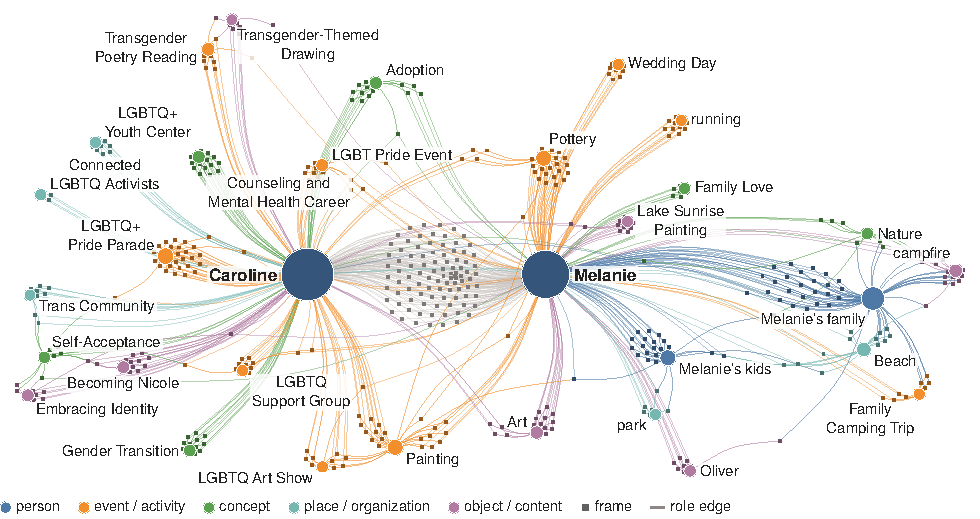
\includegraphics[width=\textwidth]{figures/graph_conv26_network.pdf}
\caption{The 32 anchors with the most frames in the conv-26 hypergraph and the 448 frames that join them. Anchors are colored by type and sized by frame count, and frames take the color of their nearest topic.}
\label{fig:graph-conv26}
\end{figure}

We built this graph with graph indexing and AutoDream enabled, using Claude
Haiku 5.5 for extraction and Cohere Embed v4 for embeddings instead of the
models described in \Cref{sec:exp-setup}.

\section{Additional results}
\label{app:results}

This appendix gives the full tables behind \Cref{fig:res-ablation,fig:res-baselines,fig:res-agent,fig:res-alfworld-types,fig:res-cost}.
Accuracy and success rates are percentages, and differences are in points.

\subsection{User memory}
\label{app:results-user}

\Cref{tab:lme} lists the LongMemEval-S accuracy of every system, judged like LoCoMo
by \texttt{gpt-4o-mini} with majority-of-3 voting. It reports M0, M1, and M2, so it complements the LoCoMo
ablation of \Cref{tab:locomo}. \Cref{tab:docqa} gives the results on the three document QA tasks of
MemoryAgentBench. SHDocQA and MHDocQA ask single-hop and multi-hop questions about
long documents and use substring matching on 100 questions each, and DetectiveQA uses
letter exact matching on 71 questions. The document QA runs use M1, with AutoDream disabled by experimental choice.

We ran HyperMem ourselves with its original settings unchanged, and all HyperMem
results in this paper come from these runs. On LoCoMo, our run reaches 91.0\%,
below the 92.7\% reported by \citet{hypermem}.

\suppressfloats[t]
\begin{table}[t]
\centering
\begin{minipage}[t]{0.43\textwidth}
\centering
\caption{LongMemEval-S accuracy (\%) on the evaluated 300 questions.}
\label{tab:lme}
\small
\begin{tabular}{lc}
\toprule
Method & Accuracy \\
\midrule
mem0        & 56.3 \\
A-Mem       & 45.0 \\
MemoryBank  & 39.7 \\
Graphiti    & 23.0 \\
HyperMem    & 58.3 \\
\midrule
MIRIX-1.0 (M0)              & 58.8 \\
\ours\ (M1, graph)           & {70.0} \\
\ours\ (M2, graph $+$ dream) & \textbf{72.6} \\
\bottomrule
\end{tabular}
\end{minipage}\hfill
\begin{minipage}[t]{0.53\textwidth}
\centering
\caption{Document QA accuracy (\%). \ours uses M1, with AutoDream disabled.}
\label{tab:docqa}
\small
\begin{tabular}{lccc}
\toprule
Method & SHDoc & MHDoc & Detective \\
\midrule
mem0        & 48.0 & 22.0 & 53.5 \\
A-Mem       & 14.0 & 20.0 & 62.0 \\
MemoryBank  & 34.0 & 28.0 & \textbf{67.6} \\
Graphiti    & 50.0 & 43.0 & 54.9 \\
HyperMem    & 52.0 & 49.0 & 66.2 \\
\ours\ & \textbf{83.0} & \textbf{71.0} & 64.8 \\
\bottomrule
\end{tabular}
\end{minipage}
\end{table}

On LongMemEval-S the graph increment of 11.2 points accounts for most of the
14.3-point margin over HyperMem. The
flat configuration M0 reaches 58.8\%, close to HyperMem at 58.3\% and mem0 at 56.3\%,
while M1 reaches 70.0\% and M2 72.6\%, 14.3 points above HyperMem. On SHDocQA and MHDocQA, HyperMem is the strongest baseline, and M1 leads it by 31.0
and 22.0 points. DetectiveQA is the exception.
MemoryBank leads with 67.6\%, followed by HyperMem with 66.2\% and M1 with 64.8\%.
A-Mem varies the most across the three document tasks, from 14.0\% on SHDocQA to
62.0\% on DetectiveQA.

\Cref{tab:memcd-gen} completes the MemoryCD results of \Cref{tab:memcd-summ} with
review generation for the same 100 users in the Home\_and\_Kitchen domain. In both
MemoryCD tables, cross-domain memory comes from the other three Amazon domains, and
single-domain memory and testing use the same domain, so the cross-domain setting asks
whether preferences stored for other products carry over to a new domain. R-1, R-L,
B-4, and BERT denote ROUGE-1, ROUGE-L, BLEU-4, and BERTScore-F1, higher is better, and
bold marks column maxima, including ties.

\begin{table}[H]
\centering
\caption{Review generation on MemoryCD, with the users and domains of \Cref{tab:memcd-summ}.}
\label{tab:memcd-gen}
\small
\begin{tabular}{lcccc|cccc}
\toprule
& \multicolumn{4}{c|}{Cross-domain} & \multicolumn{4}{c}{Single-domain} \\
\cmidrule(lr){2-5}\cmidrule(lr){6-9}
Method & R-1 & R-L & B-4 & BERT & R-1 & R-L & B-4 & BERT \\
\midrule
Long-context & .2842 & .1434 & .0092 & .8521 & .2865 & .1455 & .0105 & .8520 \\
RAG          & .2727 & .1354 & .0070 & .8484 & .2818 & .1407 & .0078 & .8498 \\
mem0         & .2783 & .1432 & .0087 & .8514 & .2780 & .1391 & .0083 & .8502 \\
A-Mem        & .2836 & .1434 & .0094 & .8520 & .2857 & .1445 & .0101 & .8517 \\
MemoryBank   & .2799 & .1424 & .0073 & .8505 & .2835 & .1424 & .0089 & .8514 \\
Graphiti     & .2717 & .1379 & .0083 & .8496 & .2808 & .1441 & .0099 & .8512 \\
\ours\  & \textbf{.2846} & \textbf{.1491} & \textbf{.0108} & \textbf{.8544} & \textbf{.2868} & \textbf{.1487} & \textbf{.0106} & \textbf{.8539} \\
\bottomrule
\end{tabular}
\end{table}

\ours has the highest value in every column of both settings, but the margins are
small. In the cross-domain setting its ROUGE-L of .1491 is .0057 above the next best,
.1434 for Long-context and A-Mem, and its BLEU-4 of .0108 is .0014 above A-Mem.
BERTScore spans at most .006 across all systems in either setting. In the
single-domain setting the margins shrink further, for example .2868 against .2865
for Long-context on ROUGE-1. 

\subsection{Agent memory}
\label{app:results-agent}

\Cref{tab:alfworld-proc} breaks down the ALFWorld success rates of \Cref{fig:res-agent}
by task type for both backbones, with the number of held-out episodes of each type in
parentheses, 134 in total. \textbf{All} is the overall success rate, given as the mean
and the sample standard deviation over three runs. Average steps are taken over all
episodes, with a cap of 50 steps, and over successful episodes only, and lower is
better. For each model, bold marks the best of the three memory methods.
\Cref{fig:res-alfworld-types} plots the GPT-6 Luna rows.

\suppressfloats[t]
\begin{table}[t]
\centering
\caption{ALFWorld success by task type (episodes per type in parentheses) and average steps, over three runs.}
\label{tab:alfworld-proc}
\small
\setlength{\tabcolsep}{3.3pt}
\begin{adjustbox}{max width=\textwidth}
\begin{tabular}{llccccccccc}
\toprule
 & & \multicolumn{7}{c}{Success rate (\%)} & \multicolumn{2}{c}{Avg.\ steps} \\
\cmidrule(lr){3-9} \cmidrule(lr){10-11}
Model & Method & Pick (24) & Look (18) & Clean (31) & Heat (23) & Cool (21) & Pick Two (17) & All & all & succ. \\
\midrule
\multirow{4}{*}{GPT-6 Luna}
  & No memory     & 83.3 & 85.2 & 60.2 & 47.8 & 81.0 & 64.7 & 69.4$\pm$0.7 & 25.2 & 14.2 \\
  & ReasoningBank & 70.8 & 66.7 & 65.6 & 63.8 & 82.5 & 49.0 & 66.9$\pm$2.8 & 26.4 & 14.7 \\
  & AWM           & 77.8 & 77.8 & 64.5 & \textbf{75.4} & \textbf{88.9} & 58.8 & 73.6$\pm$1.9 & 23.2 & 13.6 \\
  & \ours         & \textbf{79.2} & \textbf{83.3} & \textbf{74.2} & 73.9 & 85.7 & \textbf{60.8} & \textbf{76.4$\pm$6.2} & \textbf{21.9} & \textbf{13.2} \\
\midrule
\multirow{4}{*}{GPT-5.6 Luna}
  & No memory     & 73.6 & 63.0 & 37.6 & 50.7 & 66.7 & 37.3 & 54.2$\pm$1.1 & 31.6 & 16.1 \\
  & ReasoningBank & \textbf{75.0} & 50.0 & 50.5 & 53.6 & 46.0 & 31.4 & 52.2$\pm$0.7 & 31.4 & 14.4 \\
  & AWM           & 69.4 & 61.1 & 44.1 & \textbf{63.8} & 65.1 & \textbf{47.1} & 58.0$\pm$2.8 & 29.9 & 15.3 \\
  & \ours         & 69.4 & \textbf{75.9} & \textbf{54.8} & \textbf{63.8} & \textbf{66.7} & 39.2 & \textbf{61.7$\pm$14.0} & \textbf{26.8} & \textbf{12.4} \\
\bottomrule
\end{tabular}
\end{adjustbox}
\end{table}

With GPT-6 Luna, \ours is the best of the three memory methods on four of the six
task types, Pick, Look, Clean, and Pick Two, and AWM is ahead on Heat and Cool.
Against no memory, Clean gains 14.0 points, Heat 26.1, and Cool 4.7, while Pick,
Look, and Pick Two lose 4.1, 1.9, and 3.9 points.
With GPT-5.6 Luna, \ours leads the memory methods on Look, Clean, and Cool and ties
AWM on Heat at 63.8\%, while ReasoningBank is ahead on Pick and AWM on Pick Two. With
both backbones \ours takes the fewest steps, 21.9 and 26.8 over all episodes and 13.2
and 12.4 over successful ones, but its overall standard deviation of 14.0 points with
GPT-5.6 Luna is the largest in the table.

\Cref{tab:webshop-proc} gives the same breakdown for WebShop with GPT-6 Luna over the
five product categories of the 140 test instructions, with a cap of 15 steps. A
WebShop episode succeeds when its reward is 1, and bold again marks the best of the
three memory methods.

\begin{table}[H]
\centering
\caption{WebShop success by product category and average steps with GPT-6 Luna, over three runs.}
\label{tab:webshop-proc}
\small
\setlength{\tabcolsep}{3.3pt}
\begin{adjustbox}{max width=\textwidth}
\begin{tabular}{lcccccccc}
\toprule
& \multicolumn{6}{c}{Success rate (\%)} & \multicolumn{2}{c}{Avg.\ steps} \\
\cmidrule(lr){2-7} \cmidrule(lr){8-9}
Method & Fashion (30) & Beauty (21) & Electronics (29) & Garden (32) & Grocery (28) & All & all & succ. \\
\midrule
No memory & 54.4 & 31.7 & 21.8 & 19.8 & 32.1 & 31.9$\pm$1.8 & 7.9 & 6.2 \\
ReasoningBank & 43.3 & 33.3 & 12.6 & 17.7 & 23.8 & 25.7$\pm$3.8 & 10.2 & 6.9 \\
AWM & 53.3 & 31.7 & \textbf{28.7} & \textbf{27.1} & \textbf{38.1} & 36.0$\pm$4.3 & 9.1 & 6.9 \\
\ours & \textbf{57.8} & \textbf{39.7} & 25.3 & \textbf{27.1} & \textbf{38.1} & \textbf{37.4$\pm$2.1} & \textbf{8.2} & \textbf{6.3} \\
\bottomrule
\end{tabular}
\end{adjustbox}
\end{table}

\ours has the highest overall success, 37.4\% against 36.0\% for AWM and 31.9\%
without memory, and the smallest spread among the memory methods, 2.1 points. Its margins over AWM are 4.5 points on Fashion and 8.0 on Beauty. It matches AWM on
Garden and Grocery, at 27.1\% and 38.1\%, and trails it by 3.4 points on Electronics. ReasoningBank falls below no memory overall, as it does on ALFWorld with both
backbones, and on four of the five categories. All three memory methods take more
steps over all episodes than no memory, 8.2 to 10.2 against 7.9, and \ours takes the
fewest of the three.

\subsection{Costs}
\label{app:results-cost}

\Cref{tab:eff-docqa} gives the measurements behind \Cref{fig:res-cost}. Ingest is the
total wall-clock time in seconds, and Ans./q is the mean time to retrieve and answer
one question. Answer tokens sum input and output over all questions, where K and M
denote thousands and millions. Graph size counts Neo4j nodes and edges and excludes
the evidence store. M0 builds no graph, and for HyperMem the column names its index type instead of a size. None of these measurements includes
AutoDream, so they characterize M1 and not the full M2 system.

\suppressfloats[t]
\begin{table}[t]
\centering
\caption{Cost of memory for HyperMem, M0, and M1, all without AutoDream.}
\label{tab:eff-docqa}\label{tab:eff-conv}
\small
\begin{tabular}{llcccc}
\toprule
Benchmark & Method & Ingest (s) & Ans./q (s) & Ans.\ tok. & Graph (nodes/edges) \\
\midrule
\multirow{3}{*}{SHDoc}
 & HyperMem       & 5{,}665 & 10.55 & 3.79M & hypergraph \\
 & MIRIX-1.0 (M0) & 6{,}227 & 3.76 & 763K & none \\
 & \ours\ (M1)    & 23{,}784 & 5.45 & 1.40M & 29{,}341 / 33{,}526 \\
\midrule
\multirow{3}{*}{MHDoc}
 & HyperMem       & 11{,}031 & 10.65 & 3.06M & hypergraph \\
 & MIRIX-1.0 (M0) & 13{,}792 & 7.46 & 1.23M & none \\
 & \ours\ (M1)    & 55{,}301 & 9.01 & 1.33M & 49{,}046 / 55{,}288 \\
\midrule
\multirow{3}{*}{Detective}
 & HyperMem       & 11{,}653 & 13.05 & 0.35M & hypergraph \\
 & MIRIX-1.0 (M0) & 10{,}321 & 5.11 & 706K & none \\
 & \ours\ (M1)    & 39{,}491 & 7.24 & 1.16M & 36{,}987 / 46{,}651 \\
\midrule
\multirow{2}{*}{LoCoMo}
 & HyperMem     & 69{,}467 &  9.70 & 16.5M & hypergraph \\
 & \ours\ (M1)  & 21{,}416 &  5.46 & 15.7M & 23{,}820 / 32{,}394 \\
\midrule
\multirow{2}{*}{LongMemEval-S}
 & HyperMem     & 170{,}224 & 10.73 & 4.10M & hypergraph \\
 & \ours\ (M1)  & 70{,}626 & 10.10 & 4.02M & 181{,}131 / 205{,}428 \\
\bottomrule
\end{tabular}
\end{table}

\Cref{tab:eff-docqa} shows where graph construction costs time. On the three document tasks, M1
ingests 3.8 to 4.0 times more slowly than M0 and 3.4 to 5.0 times more slowly than
HyperMem. On the conversational benchmarks the order reverses, and M1 needs 21{,}416\,s
for LoCoMo against 69{,}467\,s for HyperMem and 70{,}626\,s for LongMemEval-S against
170{,}224\,s. Answering is faster for M1 than for HyperMem on all five benchmarks, by between 0.63\,s per question on LongMemEval-S and 5.81\,s on DetectiveQA, although M0 answers
the document questions faster still. M1 uses fewer answer tokens than HyperMem on four
benchmarks and more on DetectiveQA, 1.16M against 0.35M. Its graphs range from 23{,}820
nodes and 32{,}394 edges for LoCoMo to 181{,}131 nodes and 205{,}428 edges for
LongMemEval-S.

For \Cref{tab:agent-token-consumption}, training covers actor interactions and memory
learning, and testing covers actor interactions and memory retrieval on all test
tasks, including unsuccessful ones. Counts include LLM input and output tokens, with
reasoning tokens in the output and cached tokens in the input, and exclude embedding
tokens. No memory skips training.




% \section{Full Experimental Results with Different Runs}
% \label{sec:full_experimental_results}

% \begin{table*}[!t]
% \centering
% % \resizebox{\linewidth}{!}{%
% \begin{adjustbox}{max width=\textwidth}
% \begin{tabular}{p{0.5cm}l|cccc|c}   % ← added a 1.5 cm column on the left
% \toprule
% & \textbf{Method} & \textbf{Single Hop} & \textbf{Multi-Hop} & \textbf{Open Domain} & \textbf{Temporal} & \textbf{Overall} \\
% \midrule
% \multirow{8}{*}{\rotatebox[origin=c]{90}{\textbf{gpt-4o-mini}}}
%   & A-Mem      & 39.79 & 18.85 & 54.05 & 49.91 & 48.38 \\
% & LangMem     & 62.23 & 47.92 & 71.12 & 23.43 & 58.10 \\
% & OpenAI      & 63.79 & 42.92 & 62.29 & 21.71 & 52.90 \\
% & Mem0        & 67.13 & 51.15 & 72.93 & 55.51 & 66.88 \\
% & Mem0$^g$       & 65.71 & 47.19 & \textbf{75.71} & 58.13 & 68.44 \\
% & Memobase    & 63.83 & 52.08 & 71.82 & 80.37 & 70.91 \\
% & Zep         & 74.11 & 66.04 & 67.71 & 79.76 & 75.14\\
% \cmidrule{2-7}
% & Full-Context & 80.14 & 46.89 & 58.33 & 90.49 & 77.51 \\
% \midrule
% \multirow{9}{*}{\rotatebox[origin=c]{90}{\textbf{gpt-4.1-mini}}}
%  % & Zep & 48.23 & 17.76 & 39.58 & 62.43 & 49.09 \\
%   & LangMem & 76.24 & 63.24 & 63.54 & 88.11 & 79.22 \\
% & RAG-500 & 37.94 & 37.69 & 48.96 & 61.83 & 51.62 \\
% & Mem0    & 62.41 & 57.32 & 44.79 & 66.47 & 62.47 \\
% \cmidrule{2-7}
% & \textbf{\ours-Run1}   & 85.46 & 80.06 & 64.58 & 87.16 & 83.98 \\
% & \textbf{\ours-Run2}   & 82.56 & 80.69 & 63.54 & 85.26 & 82.30 \\
% & \textbf{\ours-Run3}   & 85.46 & 85.36 & 64.58 & 91.32 & 87.34 \\
% \cmidrule{2-7}
% & Full-Context-Run1 & 88.30 & 71.74 & 72.92 & 92.98 & 86.43 \\
% & Full-Context-Run2 & 88.29 & 81.31 & 71.88 & 92.50 & 88.13 \\
% & Full-Context-Run3 & 89.01 & 80.06 & 70.83 & 92.63 & 88.00 \\
% \bottomrule
% \end{tabular}%}
% \end{adjustbox}
% \caption{LLM-as-a-Judge scores (\%, higher is better) for each question type in the \texttt{LOCOMO} dataset. As mentioned in Mem0~\citep{mem0}, as the average length in this dataset is only 9k, Full-Context is almost the upper-bound. Thus recovering the performance of Full-Context shows the advancements of \ours. For Zep, we only achieve 49.09 overall score with \texttt{gpt-4.1-mini} using the implementation from mem0, we are afraid there might be errors in their implementation, so we skip the results here.}
% \label{tab:judge_only}
% \end{table*}